\begin{figure*}
  \centering
  \begin{subfigure}[b]{\textwidth}
    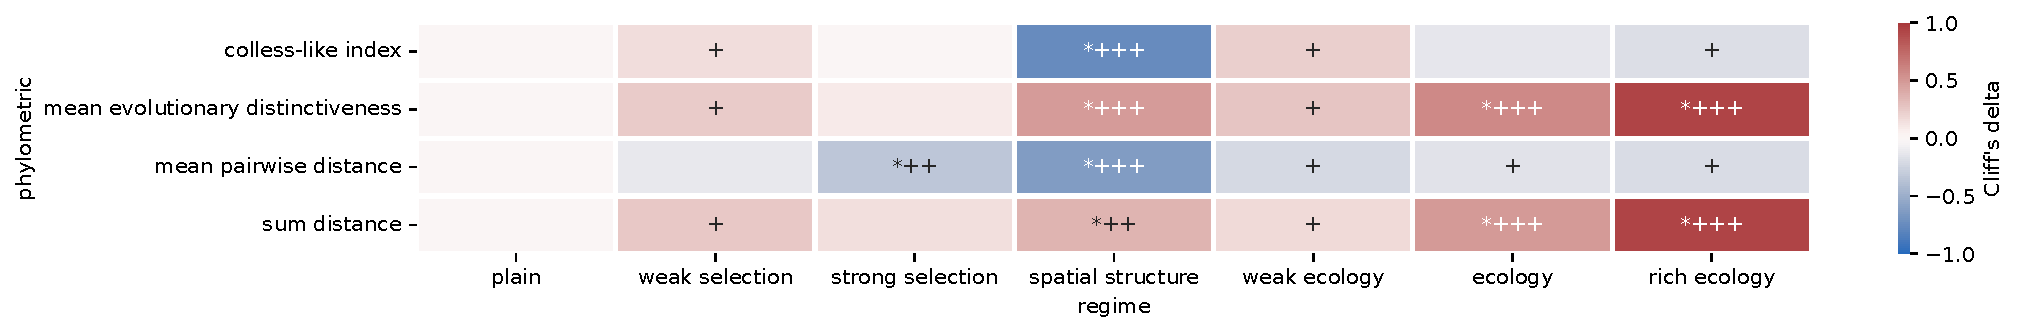
\includegraphics[width=\textwidth]{binder/binder/avida-individual/teeplots/epoch=0+mut_distn=default+viz=heatmap+x=regime+y=phylometric+ext=.pdf}
    \caption{Reference phylogeny.}
  \end{subfigure}

\begin{subfigure}[b]{\textwidth}
  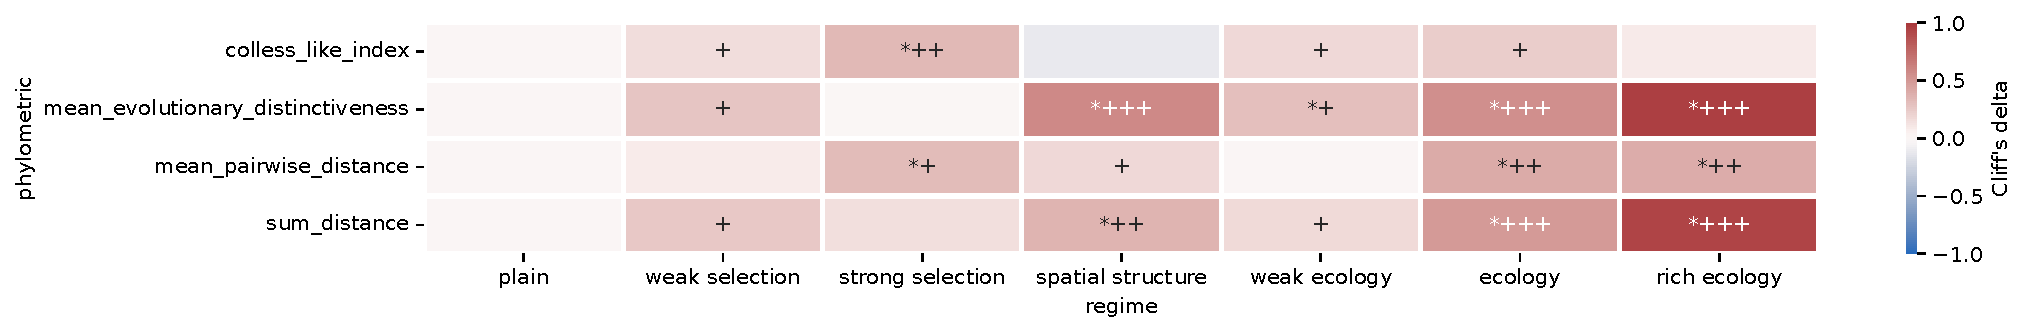
\includegraphics[width=\textwidth]{binder/binder/avida-individual/teeplots/epoch=0+mut_distn=default+resolution=100.0+viz=heatmap+x=regime+y=phylometric+ext=.pdf}
  \caption{1\% resolution reconstruction.}
\end{subfigure}

\begin{subfigure}[b]{\textwidth}
  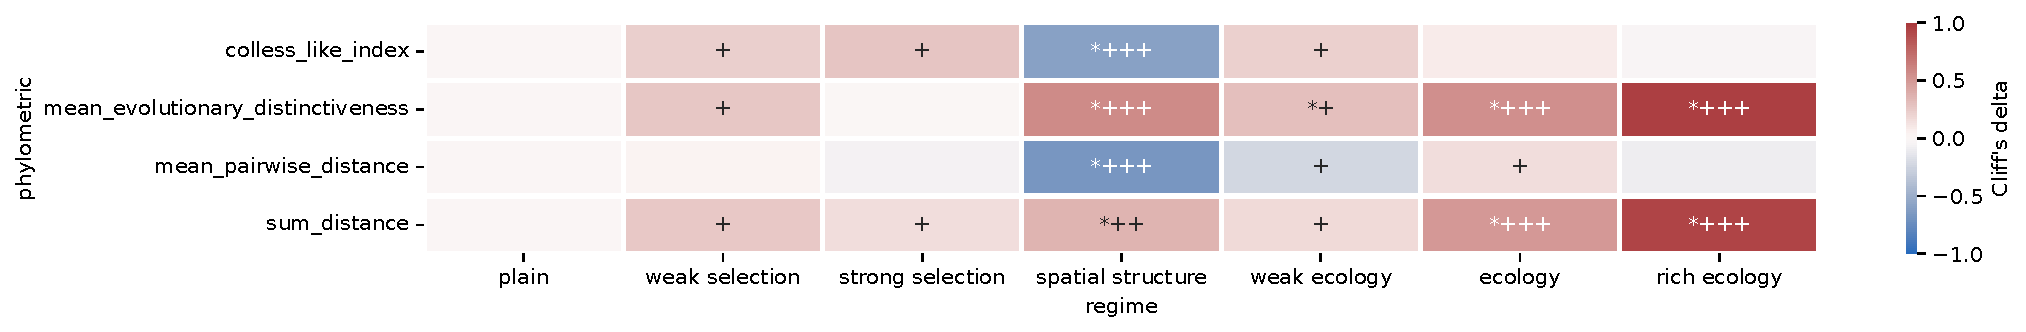
\includegraphics[width=\textwidth]{binder/binder/avida-individual/teeplots/epoch=0+mut_distn=default+resolution=33.0+viz=heatmap+x=regime+y=phylometric+ext=.pdf}
  \caption{3\% resolution reconstruction.}
\end{subfigure}

\begin{subfigure}[b]{\textwidth}
  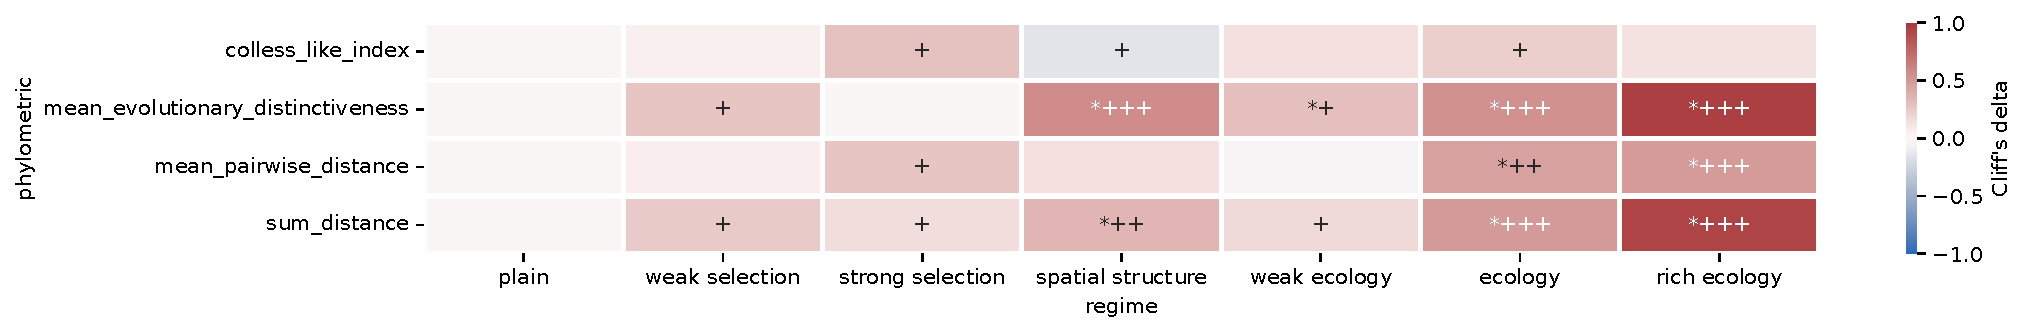
\includegraphics[width=\textwidth]{binder/binder/avida-individual/teeplots/epoch=0+mut_distn=default+resolution=10.0+viz=heatmap+x=regime+y=phylometric+ext=.pdf}
  \caption{10\% resolution reconstruction.}
\end{subfigure}

\begin{subfigure}[b]{\textwidth}
  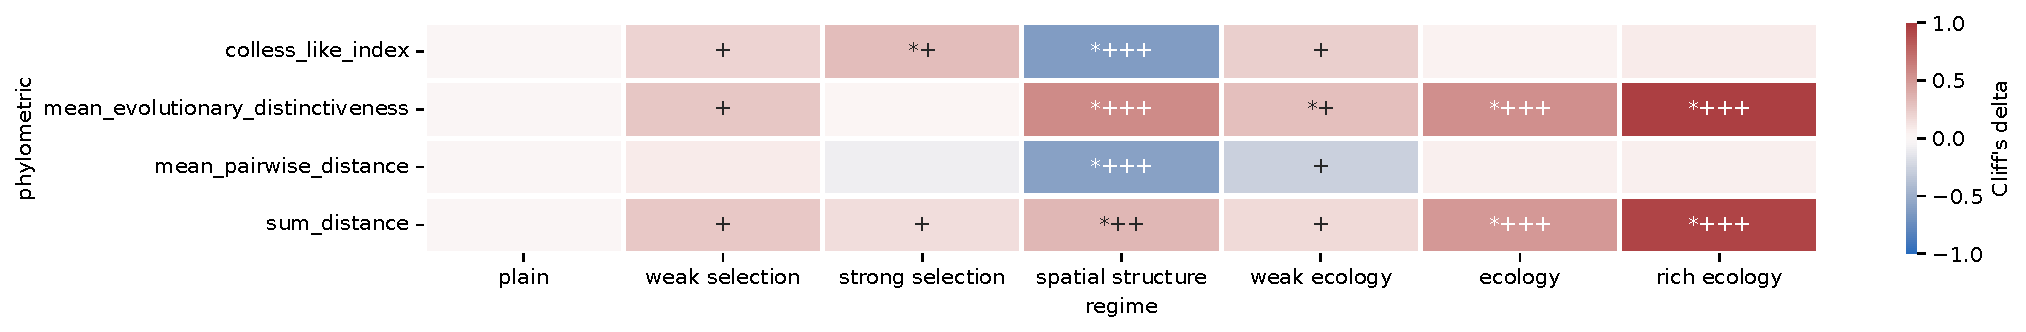
\includegraphics[width=\textwidth]{binder/binder/avida-individual/teeplots/epoch=0+mut_distn=default+resolution=3.0+viz=heatmap+x=regime+y=phylometric+ext=.pdf}
  \caption{30\% resolution reconstruction.}
\end{subfigure}

  \caption{
Tree phylometrics across surveyed evolutionary regimes, calculated on reconstructed and perfect-fidelity simulation phylogenetic records from Avida model.
Note that nonparametric effect size normalization caps out to 1.0/-1.0 past the point of complete disbributional nonoverlap.
For heatmap charts, +'s indicate small, medium, and large effect sizes using the Cliff's delta statistic and *'s indicate statistical significance at $\alpha = 0.05$ via Mann-Whitney U test.
  }
  \label{fig:reconstructed-tree-phylometrics-progressive-heatmap-avida}
\end{figure*}